#############################################################################################################################################################
\clearpage
% Therefore, the scaling effect that incremental learning has on the skill complexity $c_{j,k}$ for the skills contained in the $k$-th cluster is
%% ---
%\begin{equation}\label{eq:complexity_IL}
%	c^{(I)}_{j,k}(n) =c_0 \bar{\sigma}^{(I)}_{j,k}(n)= c_0  e^{-\alpha N_{\zeta_k} n},
%\end{equation}
%% ---
%with $r = 1$ in \eqref{eq:incremental_knowledge} since the agent has access to its own knowledge only. Eq.~\eqref{eq:complexity_IL}  is precisely the effect shown in Fig.~\ref{fig:complexity_per_cardinality} ---displayed for $n=1$---, which obeys Asm.~\ref{assumption:fundamental_complexity} and \ref{assumption:exponential_decrease}.
%Let, for simplicity, $\epsilon= e^{-5}$ then
%% ---
%\begin{equation}\label{eq:complexity_IL}
%	c^{(I)}_{j,k} = 5 \tau,
%\end{equation}
%% ---
%where $\tau = \left( \alpha (N_{\zeta_k}+ 1)\right)^{-1}.$. 
The total number of trial episodes $ C_k $ that an agent following an incremental learning strategy needs to learn the $N_{\mathcal{Z}_k}$ skills in a cluster $ \mathcal{Z}_k $ is given by
% ---
%\begin{align}
%	\begin{split}
	%		C^{(I)}_k &= \sum^{N_\mathcal{S}/N_\mathcal{K}}_{j=1} c_0 \cdot e^{-\alpha \cdot {^kN_{j}}} = \sum^{N_\mathcal{S}/N_\mathcal{K}}_{j=1}c_0 \cdot e^{-\alpha {^{k}\cancelto{j-1}{N_{j}}}}\\
	%		&= c_0 \sum^{N_\mathcal{S}/N_\mathcal{K}}_{j=1} e^{-\alpha (j-1)}.
	%	\end{split}
%\end{align}
\begin{align}\label{eq:total_episodes_incremental}
	\begin{split}
		C^{(I)}_k &= \sum^{N_{\mathcal{Z}_k}}_{j=1} c^{(I)}_{j,k}  \\
		&= \sum^{{\mathcal{Z}_k}}_{j=1} c_0 \cdot  \bar{\sigma}_{j,k}  = \sum^{{\mathcal{Z}_k}}_{j=1} c_0 e^{-\alpha {\cancelto{j-1}{N_{j,k}}}}\\
		&= c_0 \sum^{{\mathcal{Z}_k}}_{j=1} e^{-\alpha (j-1)}=c_0 \frac{1 - e^{-\alpha N_k}}{1 - e^{-\alpha}}.
	\end{split}
\end{align}
% ---
Eq.~\eqref{eq:total_episodes_incremental} is the closed form of a geometric series, where the equality $N_{j.k} = j-1$ comes from the fact that when learning the $j$-th skill in the cluster, $j-1$ skills have already been learned and their knowledge is contained in $\mathcal{\zeta}_k$. Likewise, the total number of episodes to learn the skills in all the $ N_\mathcal{Z} $ clusters is
%\begin{align}\label{eq:complexity_incremental_single}
%	\begin{split}
	%	C^{(I)} &= N_\mathcal{K} \cdot c_0 \frac{1 - e^{-\alpha \frac{N_\mathcal{S}}{N_\mathcal{K}}}}{1 - e^{-\alpha}}\\
	%&= N_\mathcal{K} \cdot c_0 \frac{1 - \bar{\sigma}^{(I)}}{1 - e^{-\alpha}}.
	%	\end{split}
%
%\end{align}
%\begin{align}\label{eq:complexity_incremental_single}
%	\begin{split}
	%		C_\mathcal{S}^{(I)} &= N_\mathcal{K} \cdot c_0 \frac{1 - e^{-\alpha \frac{N_\mathcal{S}}{N_\mathcal{K}}}}{1 - e^{-\alpha}}\\ 
	%		&= N_\mathcal{K} \cdot c_0 \frac{1 - \bar{\sigma}_k^{(I)}}{1 - e^{-\alpha}}.
	%	\end{split}
%\end{align}
\begin{align}\label{eq:complexity_incremental_single}
	\begin{split}
		C_\mathcal{S}^{(I)} &= \sum_{k=1}^{N_\mathcal{Z}} C^{(I)}_k\\
		&= N_\mathcal{Z} \cdot c_0 \frac{1 - e^{-\alpha N_k}}{1 - e^{-\alpha}}\\ 
		&= N_\mathcal{Z} \cdot c_0 \frac{1 - \bar{\sigma}_k^{(I)}}{1 - e^{-\alpha}}.
	\end{split}
\end{align}
% ---
with $ \overbrace{\bar{\sigma}^{(I)}_k = e^{- \alpha\lvert  \mathcal{Z}_k \rvert} = e^{-\alpha N_k}}^{\text{isn't this supposed to be 0?}} $ representing the knowledge remaining after learning all the skills in a cluster. If $ m $ robots are available, the learning load is distributed, with each robot taking care of learning $ \frac{N_k}{m} $ skills in parallel with the rest. Under such conditions, the total number of episodes is simply
% ---
\begin{align}\label{eq:complexity_incremental_parallel}
	\begin{split}
		{}^{\lvert \rvert}C_\mathcal{S}^{(I)} &= m \left( N_\mathcal{Z} \cdot c_0 \frac{1 - e^{-\alpha \frac{N_k}{m}}}{1 - e^{-\alpha}}\right) \\&= m \left( N_\mathcal{Z} \cdot c_0 \frac{1 - \left(\bar{\sigma}^{(I)}_k\right)^{\frac{1}{m}} }{1 - e^{-\alpha}} \right) \\
		&= m \cdot N_\mathcal{Z} \cdot c_0 \frac{1 - \bar{\sigma}^{(I)}_m}{1 - e^{-\alpha}} 	
	\end{split}	
\end{align}
%---
\begin{table*}[htbp!]
	\begin{center}
		\captionof{table}{The total complexity of the different learning schemes.} \label{tab:method_comparison}
		\begin{tabular}{|c|c|c|c| } 
			\multicolumn{4}{c}{\cellcolor{black!25} $c_{j,k_\mathcal{T}}=c_0\left[1- \sum\limits_{k \in \mathcal{K} \setminus k_\mathcal{T}}\beta_k \left( 1 - \bar{\sigma}_{j,k} \right)\right] \left(e^{-\alpha N_{j,k_\mathcal{T}}} \right)^r$}\\
			\hline
			\cellcolor{black!25} & \textbf{Incremental} & \textbf{Transfer} & \textbf{Collective}\\
			\cellcolor{black!25} & $r=1, \quad \beta_k=0$ & $r=1$ & $r=m, \quad \mathcal{K} \setminus k_\mathcal{T}=\emptyset, \quad N_{j,k_\mathcal{K}} = N_j$\\
			\hline 
			Single & $ C_\mathcal{S}^{(I)} = N_\mathcal{K} \cdot c_0 \frac{1 - e^{-\alpha \frac{N_\mathcal{S}}{N_\mathcal{K}}}}{1 - e^{-\alpha}}  $ 
			& $C_\mathcal{S}^{(T)}= \left[1 - \frac{\left(1+N_\mathcal{K}\right)}{2}\beta \left(1-\bar{\sigma}\right)\right] C_\mathcal{S}^{(I)}$& \multirow{2}{*}{${^{\vert \lvert}}C_\mathcal{S}^{(C)} = m \cdot c_0 \frac{1 - e^{-\alpha N_\mathcal{S}}}{1 - e^{-\alpha m}}$}\\
			%\hline
			Parallel & $ {^{\vert \lvert}}C_\mathcal{S}^{(I)} = m \cdot N_\mathcal{K} \cdot c_0 \frac{1 - e^{-\alpha \frac{N_\mathcal{S}}{m \cdot N_\mathcal{K}}}}{1 - e^{-\alpha}}  $ 
			& ${^{\vert \lvert}}C_\mathcal{S}^{(T)} = \left[1 - \frac{\left(1+N_\mathcal{K}\right)}{2}\beta \left(1-\bar{\sigma}_m\right)\right] {^{\vert \lvert}}C_\mathcal{S}^{(I)}$ & \\
			\hline
		\end{tabular}
	\end{center}
	%\label{tab:method_comparison}
\end{table*}
% ---------------------------------------------------------------------------------------------------
\subsubsection{\textbf{Transfer learning (TL)}}

%\begin{figure}[!h]
%	\centering
%	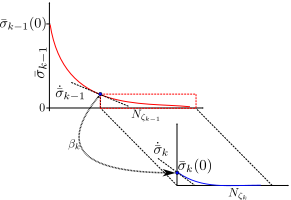
\includegraphics[width=0.9\columnwidth]{fig/effect_transfer_learning.pdf}
%	\caption{The effect of transfer learning.}
%	\label{fig:effect_transfer_learning}
%\end{figure}
%---
%TL represents the exchange of knowledge from the skills learned in different \emph{origin} clusters $\mathcal{O}$ to the skills that will be learned in a \emph{target} cluster $\mathcal{T}$, see Fig.~\ref{fig:incremental_transfer_similarity}. In general, the effect that TL has on the skills of another cluster is the reduction of the total remaining knowledge to be learned. Referring to \eqref{eq:differential_incremental_knowledge} and \eqref{eq:incremental_knowledge}, it means that its initial condition when $N_{j,k} = 0$ will be reduced (Fig.~\ref{fig:effect_transfer_learning}). Considering $\mathcal{K} = \{ \mathcal{Z}_k \}^{N_\mathcal{Z}}_{k=1}$ to be the set of all available clusters of knowledge (see Fig.~\ref{fig:cluster_knowledge_transfer}), the TL effect can be modeled as follows
Considering $\mathcal{K} = \{ \mathcal{Z}_k \}^{N_\mathcal{Z}}_{k=1}$ to be the set of all available skill clusters (see Fig.~\ref{fig:cluster_knowledge_transfer}), TL represents the exchange of knowledge from the skills learned in different \emph{origin} clusters $\mathcal{O} = \{ \mathcal{Z}_1,\mathcal{Z}_2,\ldots,\mathcal{Z}_{k-1} \}$ to the skills that will be learned in a \emph{destination} cluster $\mathcal{Z}_k$, see Fig.~\ref{fig:incremental_transfer_similarity}. In general, the effect that TL has on the skills of another cluster is the reduction of the total remaining knowledge to be learned. Referring to \eqref{eq:differential_incremental_knowledge} and \eqref{eq:incremental_knowledge}, it means that its initial condition when $N_{j,k} = 0$ will be reduced (Fig.~\ref{fig:effect_transfer_learning}). The TL effect can be modeled as follows
% ---
\begin{subequations}\label{eq:joint_cartesian_acceleration}
	\begin{equation}\label{eq:joint_cartesian_acceleration_child}
		\dot{\bar{\sigma}}^{(T)}_{j,k} = -\alpha  \cdot N_{j,k}
	\end{equation}    
	\begin{equation}\label{eq:joint_cartesian_acceleration_parent}
		\bar{\sigma}^{(T)}_{j,k}(0) = 1 - \sum\limits_{c = 1}^{k-1}\beta_{c} \left( 1 - \bar{\sigma}_{c} \right),~\bar{\sigma}_{c=0} = 1
	\end{equation}
\end{subequations}
% ---
Implying that the remaining knowledge under transfer learning is
% ---
\begin{align}
	\begin{split}
		\bar{\sigma}^{(T)}_{j,k} 
		&= \underbrace{\left[1- \sum\limits_{c = 0}^{k-1}\beta_{c} \left( 1 - \bar{\sigma}_{c} \right)\right]}_{\text{Transferred knowledge}} e^{-\alpha N_{j,k}}
	\end{split}
\end{align}
% ---
where $0<\beta_{c} < 1$ is the transfer coefficient from the different origin clusters $\mathcal{Z}_{c}$ to the target cluster $\mathcal{Z}_{k}$\footnote{\textcolor{red}{Once again, since there is no inter-agent exchange of knowledge, $ r = 1 $ in this case.}}. Assuming that the origin clusters have unique knowledge contributions to the destination cluster implies that
% ---
\begin{equation}
	\sum\limits_{c=0}^{k-1}\beta_{c} \leq 1;
\end{equation}
% ---
i.e. no redundant knowledge. Furthermore, considering Assumptions~\ref{assumption:cluster_size} and \ref{assumption:cluster_transferability},
% ---
% \begin{equation}
	%     \beta_{k_O} = \frac{1}{\text{max}\left(\left\lvert \mathcal{K} \setminus k_{T} \right\rvert,1\right)}
	% \end{equation}
\begin{equation}
	\beta_{c}=
	\begin{cases}
		1, & \text{if $\mathcal{O}  = \emptyset$}.\\
		\frac{1}{k - 1}, & \text{otherwise}.
	\end{cases}
\end{equation}
% ---
The term $ 1 - \bar{\sigma}_{c}$ represents the knowledge available from each of the different origin clusters (i.e. after their corresponding skills were learned).
% ---
% \begin{align}
	% 	\begin{split}
		% 		\bar{\sigma}^{(T)}_{j,k_\mathcal{T}} &= \left\{ e^{-\alpha \left(N_{j,k_\mathcal{T}} - \frac{1}{\alpha \cdot r}  \log\left[ 1- \sum\limits_{k\in \mathcal{K} \setminus k_\mathcal{T}}\beta_k(1 - \bar{\sigma}_{j,k}) \right] \right)}\right\}^r\\
		% 		&= \left(e^{-\alpha {N_{j,k_\mathcal{T}}}} \right)^r e^{  \log\left( 1-\sum\limits_{k_\mathcal{O} \in \mathcal{K} \setminus k_\mathcal{T}}\beta_k(1 - \bar{\sigma}_{j,k_{\mathcal{O}}}) \right) }\\
		% 		&= \underbrace{\left[1- \sum\limits_{k \in \mathcal{K} \setminus k_\mathcal{T}}\beta_k \left( 1 - \bar{\sigma}_{j,k} \right)\right]}_{\text{Transfer}} \left(e^{-\alpha N_{j,k_\mathcal{T}}} \right)^r ,
		% 	\end{split}
	% \end{align}


% \begin{align}
	% 	\begin{split}
		% 		\bar{\sigma}^{(T)}_{j,k_T} &= \left\{ e^{-\alpha \left(N_{j,k_T} - \frac{1}{\alpha \cdot r}  \log\left[ 1- \sum\limits_{k_O\in \mathcal{K} \setminus k_T}\beta_{k_O}\left(1 - \bar{\sigma}_{j,k_O}\right) \right] \right)}\right\}^r\\
		% 		&= \left(e^{-\alpha {N_{j,k_T}}} \right)^r e^{ \log\left( 1-\sum\limits_{k_O \in \mathcal{K} \setminus k_T}\beta_{k_O}\left(1 - \bar{\sigma}_{j,k_O}\right) \right) }\\
		% 		&= \underbrace{\left[1- \sum\limits_{k_O \in \mathcal{K} \setminus k_T}\beta_{k_O} \left( 1 - \bar{\sigma}_{j,k_O} \right)\right]}_{\text{Transfer}} \left(e^{-\alpha N_{j,k_T}} \right)^r ,
		% 	\end{split}
	% \end{align}

\begin{align}
	\begin{split}
		\bar{\sigma}^{(T)}_{j,k_T} &= \left\{ e^{-\alpha \left(N_{j,k_T} - \frac{1}{\alpha \cdot r}  \log\left[ 1- \sum\limits_{k_O\in \mathcal{K} \setminus k_T}\beta_{k_O}\left(1 - \bar{\sigma}_{k_O}\right) \right] \right)}\right\}^r\\
		&= \left(e^{-\alpha {N_{j,k_T}}} \right)^r e^{ \log\left( 1-\sum\limits_{k_O \in \mathcal{K} \setminus k_T}\beta_{k_O}\left(1 - \bar{\sigma}_{k_O}\right) \right) }\\
		&= \underbrace{\left[1- \sum\limits_{k_O \in \mathcal{K} \setminus k_T}\beta_{k_O} \left( 1 - \bar{\sigma}_{k_O} \right)\right]}_{\text{Transfer}} \left(e^{-\alpha N_{j,k_T}} \right)^r ,
	\end{split}
\end{align}
% ---
\begin{align}
	\begin{split}
		\bar{\sigma}^{(T)}_{j,k} 
		&= \underbrace{\left[1- \sum\limits_{O = 0}^{k-1}\beta_{O} \left( 1 - \bar{\sigma}_{O} \right)\right]}_{\text{Transfer}} \left(e^{-\alpha N_{j,k}} \right)
	\end{split}
\end{align}

\begin{align}
	\begin{split}
		^{\lvert \lvert}\bar{\sigma}^{(T)}_{j,k} 
		&= \underbrace{\left[1- \sum\limits_{O = 0}^{k-1}\beta_{O} \left( 1 - \bar{\sigma}_{O} \right)\right]}_{\text{Transfer}} \left(e^{-\alpha N_{j,k}/} \right)
	\end{split}
\end{align}

% and $ \bar{\sigma}_{j,k} = \bar{\sigma}_m $. Where $ \bar{\sigma}_m $ represents the knowledge collected from the other clusters; i.e.
% % ---
% \begin{equation}
	% 	\bar{\sigma}_m = e^{-\alpha \frac{N_\mathcal{S}}{m N_\mathcal{K}}}.
	% \end{equation}
%---
% \begin{figure}[!h]
	% 	\centering
	% 	\includegraphics[width=0.99\columnwidth]{tex/fig/single_transfer_knowledge.pdf}
	% 	\caption{Knowledge sharing in transfer learning. A single agent leverages previously acquired knowledge from other learned skills in the current and previously learned clusters.}
	% 	\label{fig:single_transfer_knowledge}
	% \end{figure}
% ---
\begin{figure}[!h]
	\centering
	\includegraphics[width=0.99\columnwidth]{fig/single_transfer_complexity.pdf}
	\caption{Skill complexity is reduced further by the effect of transfer learning as more clusters are visited.}
	\label{fig:single_transfer_complexity}
\end{figure}
% ---
In TL, the skill complexity in the destination cluster $\mathcal{Z}_k$ is then given by
% ---
\begin{equation}
	c^{(T)}_{j,k} = c_0 \cdot \bar{\sigma}^{(T)}_{j,k},
\end{equation}
% ---
see Fig.~\ref{fig:single_transfer_complexity}. Notice that as the number of seen clusters increases, the starting complexity for the skills in the target cluster is reduced even further. Consequently, similar to incremental learning, the number of trial episodes to learn the skills in the $\mathcal{Z}_k$ cluster is
% ---
\begin{align}\label{eq:complexity_transfer_single}
	C_{k}^{(T)} &= \left[1 - \sum_{c=0}^{k-1}\beta_{c} \left(1-\bar{\sigma}^{(I)}_{c}\right)\right]  \cdot  c_0 \frac{1 - e^{-\alpha N_k}}{1 - e^{-\alpha}}
\end{align}
% ---

and the total number of trial episodes required to learn all the skills in the $N_\mathcal{Z}$ clusters is\footnote{This corresponds to an arithmetic series.¸}
% ---
\begin{align}\label{eq:complexity_transfer_single}
	C_\mathcal{S}^{(T)} &= \sum_{k=1}^{N_\mathcal{Z}} C_{k}^{(T)}\\
	&= \left[1 - \frac{\left(1+N_\mathcal{Z}\right)}{2}\beta_c \left(1-\bar{\sigma}^{(I)}_k\right)\right] N_\mathcal{Z} \cdot  c_0 \frac{1 - e^{-\alpha N_k}}{1 - e^{-\alpha}}\\
	&= \left[1 - \frac{\left(1+N_\mathcal{Z}\right)}{2}\beta_c \left(1-\bar{\sigma}^{(I)}_k\right)\right] N_\mathcal{Z} \cdot  c_0 \frac{1 - \bar{\sigma}^{(I)}_k}{1 - e^{-\alpha}}	
\end{align}
% ---
Furthermore, if $ m $ robots can be used in parallel to learn the skills in the clusters; then
% ---
\begin{equation}\label{eq:complexity_transfer_parallel}
	{}^{\lvert \lvert}C_\mathcal{S}^{(T)} = \left[1 - \frac{\left(1+N_\mathcal{K}\right)}{2}\beta_c \left(1-\bar{\sigma}_m\right)\right] m \cdot N_\mathcal{K}  \cdot c_0 \frac{1 - e^{-\alpha \frac{N_\mathcal{S}}{m \cdot N_\mathcal{K}}}}{1 - e^{-\alpha}},
\end{equation}

\begin{tcolorbox}
	\begin{align}
		e^{-\gamma \cdot N_j \cdot m}  &= \left[1 - \frac{\left(1+N_\mathcal{K}\right)}{2}\beta \left(1-\bar{\sigma}_m\right)\right]  \cdot m \cdot \frac{1 - e^{-\alpha \frac{N_\mathcal{S}}{m \cdot N_\mathcal{K}}}}{1 - e^{-\alpha}}\\
		\gamma &= -\frac{1}{N_j my}\text{log} \left( \left[1 - \frac{\left(1+N_\mathcal{K}\right)}{2}\beta \left(1-\bar{\sigma}_m\right)\right]  \cdot m \cdot \frac{1 - e^{-\alpha \frac{N_\mathcal{S}}{m \cdot N_\mathcal{K}}}}{1 - e^{-\alpha}}\right)
	\end{align}
\end{tcolorbox}
% ---
% ---------------------------------------------------------------------------------------------------
\subsubsection{\textbf{Collective learning (CL)}}
Finally, in collective learning the notion of cluster is redefined to be formed by all the skills learning concurrently by $m$ robots. In this setting, exchange of knowledge is possible which means that at every trial episode $n$ there is 

Finally, in collective learning the notion of cluster is not necessarily applicable anymore, thus 
$\mathcal{K} = k_\mathcal{T}$ which corresponds to the existence of only one big cluster.
% ---
\begin{align}
	\begin{split}
		\bar{\sigma}_j^{(C)} &=   \cancelto{1}{ \left[1- \sum_{k_O \in \mathcal{K} \setminus k_T}\beta_{k_O} \left( 1 - \bar{\sigma}_{k_O} \right)\right]} \left(e^{-\alpha {N_{j,k_T}}} \right)^r \\
		&= \left(e^{-\alpha N_{j,k_T}} \right)^r  = \left(e^{-\alpha N_{j}}\right)^r 
	\end{split}
\end{align}

Furthermore, now $m$ robots are learning (potentially) $m$ different skills in parallel while exchanging knowledge.
% ---
\begin{align}\label{eq:collective_knowledge}
	\begin{split}
		\bar{\sigma}_i^{(C)} &= \left({e^{-\alpha \cdot N_i}}\right)^{r}\\
		&= \left({e^{-\alpha \cdot N_i}}\right)^{m}.
	\end{split}
\end{align}
% ---
The mapping for the $i$-th skill in the universe relative to the $j$-th skill in the $k$-th cluster is
\begin{equation}
	i = (k-1)\frac{N_\mathcal{S}}{N_\mathcal{K}} + j,k
\end{equation}

%where $\alpha$ was replaced by $ 0<\gamma<<1$, which models a more effective knowledge transfer among the $m$ agents.}
Based on \eqref{eq:collective_knowledge} the scaled down skill complexity in CL is 
% ---
\begin{align}\label{eq:collective_knowledge}
\begin{split}
	^{||}c_j^{(C)} &= c_o \cdot \left({e^{-\alpha \cdot N_j}}\right)^{m}.
\end{split}
\end{align}
% ---
The total number episodes when using collective learning is given by
% ---
\begin{eqnarray}
^{||}C_\mathcal{S}^{(C)} = m \cdot C_0 \frac{1 - e^{-\alpha N_\mathcal{S}}}{1 - e^{-\alpha m}}
\end{eqnarray}
% ---
% ===================================================================================================
\subsection{Comparison}
The general skill complexity scaling based on knowledge sharing is given by the following expression
\begin{tcolorbox}
\begin{align}\label{eq:general_complexity}
	c_{j,k_T} &= c_0\left[1- \sum\limits_{k_O \in \mathcal{K} \setminus k_T}\beta_{k_O} \left( 1 - \bar{\sigma}_{k_O} \right)\right] \left(e^{-\alpha N_{j,k_T}} \right)^r
\end{align}
\end{tcolorbox}
Expression \ref{eq:general_complexity} can be re written to show the contribution of the different learning schemes as
% ---
\begin{align}
c_{j,k_T} &= c_0\underbrace{\left[1- \sum\limits_{k_O \in \mathcal{K} \setminus k_T}\beta_{k_O} \left( 1 - \bar{\sigma}^{(I)}_{k_O} \right)\right]}_{TL}\overbrace{ \left(\bar{\sigma}^{(I)}_{j,k_T} \right)^{r-1}}^{CL}\underbrace{ \left(\bar{\sigma}^{(I)}_{j,k_T} \right)}_{IL}
\end{align}
% ---
with
\begin{align}
\bar{\sigma}^{(I)}_{j,k_T}&= e^{-\alpha N_{j,k_T}},
\end{align}
where according to \eqref{eq:learning_combinations}, the effects of the different learning schemes are reflected.
% ---
\begin{equation}
c_j =
\begin{cases} 
	\text{Incremental} & \alpha\neq 0, \beta=0,  r=1 \\
	\text{Transfer} & \alpha\neq 0, \beta \neq 0, r = 1 \\
	\text{Collective} & \alpha\neq 0, \beta = 0, r=m 
\end{cases}
\label{eq:learning_combinations}
\end{equation}
From \eqref{eq:complexity_incremental_parallel} and \eqref{eq:complexity_transfer_parallel} it is clear that they differ only by the factor $ \left[1 - \frac{\left(1+N_\mathcal{K}\right)}{2}\beta \left(1-\bar{\sigma}_m\right)\right] \leq 1$, showing that TL is a scaled down version of IL. Table~\ref{tab:method_comparison} shows the comparison between the total number of trial episodes required by the three learning schemes.

% ---
The total energy and time consumption in the different learning paradigms is
% ---
\begin{align}
\begin{split}
	E^{(\star)}_{\mathcal{S}} &= e_{0} \cdot {}^{\lvert \lvert}C_\mathcal{S}^{(\star)}\\
	T^{(\star)}_{\mathcal{S}} &= \frac{\Delta t}{m} \cdot {}^{\lvert \lvert}C_\mathcal{S}^{(\star)},
\end{split}
\end{align}
% -----
with $ \star $ representing the total complexity corresponding the considered learning scheme. Fig.~\ref{fig:energy_time_learning_paradigms} shows the effect in the energy and time demand from the three different learning paradigms as a function of the number of robots learning, considering $c_0 = 100$, $P_0  = \unit[100]{W}$, $ \Delta t = \unit[300]{s}$ and $ N_\mathcal{S} = 10^6 $. In the upper panel of Fig.~\ref{fig:energy_time_learning_paradigms}, it can be seen that the transfer learning paradigm consumes less energy than the incremental one for all cluster size variations. Furthermore, there is a clear upper bound on the energy consumption for learning all skills in $\mathcal{S}$ with the increase of the number of agents $m$. This effect is due to the division of skills among the agents within a cluster; leading to agents accumulating less knowledge before moving to a new cluster. This upper bound is proportional to $c_0$. Additionally, the figure shows the performance of the robots under the collective learning paradigm to be far more efficient than the other IL and TL. On the lower pane  of Fig.~\ref{fig:energy_time_learning_paradigms}, the amount of time required by each agent to learn all skills is shown. Since the amount of time for each trial episode is fixed, we can say that the values are then proportional to the wall-clock time to learn all skills. We can see that, for all paradigms, the more agents we use the faster all skills will be learned, up to a stable point where there is no apparent performance increase by having more agents. Similar to the energy plot, TL is also more efficient than IL, but both are much less efficient than CL. We can further observe that in the collective paradigm there is a quicker saturation of the efficiency, denoting that, even with a relative small number of agents, it should be possible to learn all skills using the same wall-clock time than with a bigger number of agents. This hints at the existence of an optimal trade-off between the number of agents and the time required to learn a given number of skills.
% ---
% \begin{figure*}[!htb]
% 	\centering
% 	\hspace*{\fill}
% 	\subfloat[]{\includegraphics[width= 0.99\textwidth]{fig/energy_time_learning_paradigms.jpg}}  
% 	\hspace*{\fill}
% 	\caption[] {\label{fig:energy_time_learning_paradigms} The total energy and time demands for the different learning paradigms, considering $ N_\mathcal{S} = 10^6 $.}
% \end{figure*}
% ---
%---
\begin{figure*}[!htb]
\centering
\hspace*{\fill}
\subfloat[]{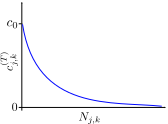
\includegraphics[width= 0.30\textwidth]{fig/complexity_incremental.pdf} \label{fig:complexity_incremental}}  
\hfill
\subfloat[]{\includegraphics[width= 0.30\textwidth]{fig/single_transfer_complexity.pdf} \label{fig:single_transfer_complexity}}  
\hfill	
\subfloat[]{\includegraphics[width= 0.30\textwidth]{fig/collective_complexity.pdf} \label{fig:collective_complexity}}
\hspace*{\fill}
\caption[] {\label{fig:energy_time_learning_paradigms} Transfer learning. \subref{fig:effect_transfer_learning} The total \subref{fig:parallel_total_energy} energy and \subref{fig:parallel_total_time} time demands for the different learning paradigms, considering $ N_\mathcal{S} = 10^6 $.}
\end{figure*}
% ---
\begin{figure*}[!htb]
\centering
\hspace*{\fill}
\subfloat[]{\includegraphics[width= 0.90\columnwidth]{fig/parallel_total_energy.pdf} \label{fig:parallel_total_energy}}  
\hfill
\subfloat[]{\includegraphics[width= 0.90\columnwidth]{fig/parallel_total_time.pdf} \label{fig:parallel_total_time}}
\hspace*{\fill}
\caption[] {\label{fig:energy_time_learning_paradigms} Transfer learning. \subref{fig:effect_transfer_learning} The total \subref{fig:parallel_total_energy} energy and \subref{fig:parallel_total_time} time demands for the different learning paradigms, considering $ N_\mathcal{S} = 10^6 $.}
\end{figure*}